\documentclass[utf8x,xcolor=pdftex,dvipsnames,table]{beamer}
\usetheme{Malmoe}  % Now it's a beamer presentation with the lisa theme!
\setbeamertemplate{footline}[page number]
\usecolortheme{beaver}
\usepackage[T1]{fontenc}
\usepackage{amsmath}
\usepackage[utf8x]{inputenc}
\usepackage{listings}

\newcommand{\superscript}[1]{\ensuremath{^{\textrm{#1}}}}

\mode<presentation>

\title{Debugging}

\author{%
\footnotesize
Frédéric Bastien \newline
\newline
\newline
Institut des algorithmes d'apprentissage de Montréal\\
Montreal Institute for Learning Algorithms\\
Université de Montréal}

\date{August 10th, Deep Learning Summer School 2015, Montréal}

\setbeamertemplate{navigation symbols}{}
\begin{document}

\begin{frame}[plain]
 \titlepage
 \vspace{-2em}
 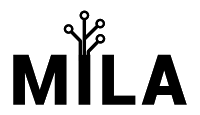
\includegraphics[width=.8in]{mila.png}
 \hfill
 
\includegraphics[width=.8in]{UdeM_logo}
\end{frame}

\begin{frame}{Slides}
  \url{http://github.com/mila-udem/summerschool2015/debug}
\end{frame}

\section{Debugging}
\begin{frame}
  \tableofcontents[currentsection]
\end{frame}

\subsection{Debugging}
\begin{frame}{Debugging}
  \begin{itemize}
  \item Error message
  \item DEBUG\_MODE
  \item theano.printing.debugprint
breakpoint op
nanguard
printop
test_value
name AssertOp
profile=True? exception_verbosity for missing memory.
%%on_opt_err, optimizer_verbose=True
  \end{itemize}
\end{frame}

\begin{frame}[fragile]
  \frametitle{Error message: code}
\lstset{language=Python,
        commentstyle=\itshape\color{blue},
        stringstyle=\color{violet},
        }
\begin{lstlisting}
import numpy as np
import theano
import theano.tensor as T
x = T.vector()
y = T.vector()
z = x + x
z = z + y
f = theano.function([x, y], z)
f(np.ones((2,)), np.ones((3,)))
\end{lstlisting}
\end{frame}

\begin{frame}[fragile]
  \frametitle{Error message: 1st part}

\lstset{language=Python,
        commentstyle=\itshape\color{blue},
        stringstyle=\color{violet},
        basicstyle=\scriptsize
        }
\begin{lstlisting}
Traceback (most recent call last):
[...]
ValueError: Input dimension mis-match.
    (input[0].shape[0] = 3, input[1].shape[0] = 2)
Apply node that caused the error:
   Elemwise{add,no_inplace}(<TensorType(float64, vector)>,
                            <TensorType(float64, vector)>,
                            <TensorType(float64, vector)>)
Inputs types: [TensorType(float64, vector),
               TensorType(float64, vector),
               TensorType(float64, vector)]
Inputs shapes: [(3,), (2,), (2,)]
Inputs strides: [(8,), (8,), (8,)]
Inputs scalar values: ['not scalar', 'not scalar', 'not scalar']
\end{lstlisting}
\end{frame}

\begin{frame}[fragile]
  \frametitle{Error message: 2st part}
HINT: Re-running with most Theano optimization
disabled could give you a back-traces when this
node was created. This can be done with by setting
the Theano flags ``optimizer=fast\_compile''. If that does not
work, Theano optimizations can be disabled with
``optimizer=None''.\newline
HINT: Use the Theano flag ``exception\_verbosity=high''
for a debugprint of this apply node.
\end{frame}


\begin{frame}[fragile]
  \frametitle{Error message: Traceback}

\lstset{language=Python,
        commentstyle=\itshape\color{blue},
        stringstyle=\color{violet},
        basicstyle=\footnotesize,
        xleftmargin=-1em
        }
\begin{lstlisting}
Traceback (most recent call last):
  File "test.py", line 9, in <module>
    f(np.ones((2,)), np.ones((3,)))
  File "/u/bastienf/repos/theano/compile/function_module.py",
       line 589, in __call__
    self.fn.thunks[self.fn.position_of_error])
  File "/u/bastienf/repos/theano/compile/function_module.py",
       line 579, in __call__
    outputs = self.fn()
\end{lstlisting}
\end{frame}


\begin{frame}[fragile]
  \frametitle{Error message: optimizer=fast\_compile}

\lstset{language=Python,
        commentstyle=\itshape\color{blue},
        stringstyle=\color{violet},
        }
\begin{lstlisting}
Backtrace when the node is created:
  File "test.py", line 7, in <module>
    z = z + y

\end{lstlisting}
\end{frame}


\begin{frame}[fragile]
  \frametitle{debugprint}

\lstset{language=Python,
        commentstyle=\itshape\color{blue},
        stringstyle=\color{violet},
        }
\begin{lstlisting}
>>> from theano.printing import debugprint
>>> debugprint(a)
Elemwise{mul,no_inplace} [@A] ''
 |TensorConstant{2.0} [@B]
 |Elemwise{add,no_inplace} [@C] 'z'
   |<TensorType(float64, scalar)> [@D]
   |<TensorType(float64, scalar)> [@E]
\end{lstlisting}
\end{frame}

%% \begin{frame}{Pylearn2}

%%   Machine Learning library aimed at researchers

%%   \begin{itemize}
%%     \item Built on top of Theano, for fast execution and use of GPU
%%     \item Easy to try variants of implemented algorithms, and to extend them (using Theano)
%%     \item Very modular, each component of the library can be used in isolation
%%     \item Experiments can be specified through a YAML config file, or by a Python script
%%     \item Scripts for visualizing weights, plot monitored values
%%   \end{itemize}
%% \end{frame}


%% \begin{frame}{libgpuarray}
%%   Goal: A common GPU $n$-dimensional array that can be reused by all projects, support for both CUDA and OpenCL.
%%   \newline \newline
%%   Motivation:
%%   \begin{itemize}
%%   \item Currently there are at least 6 different GPU arrays in Python
%%     \begin{itemize}
%%     \item CudaNdarray (Theano), GPUArray (pycuda), CUDAMatrix (cudamat), GPUArray (pyopencl), Clyther, Copperhead, ...
%%     \item There are even more if we include other languages.
%%     \end{itemize}
%%   \item They are incompatible
%%     \begin{itemize}
%%     \item None have the same properties and interface
%%     \end{itemize}
%%   \item All of them implement a subset of numpy.ndarray properties
%%   \item This is the new GPU backend on Theano
%%   \end{itemize}
%% \end{frame}


%% \begin{frame}{Project status?}
%%   \begin{itemize}
%%   \item Usable directly, but not all implementation available.
%%   \item Multiple GPUs works.
%%   \item Is the next GPU array container for Theano and is working.
%%     \begin{itemize}
%%     \item Not all Theano implementations available now.
%%     \item OpenCL misses more implementations.
%%     \item Multiple GPUs: supported in libgpuarray
%%     \item Multiple GPUs: close to get integrated in Theano.
%%     \end{itemize}
%%   \item Web site: \url{http://deeplearning.net/software/libgpuarray/}
%%   \end{itemize}
%% \end{frame}

%% \section{libgpuarray}
%% \begin{frame}
%%   \tableofcontents[currentsection]
%% \end{frame}
%% %TODO, make much shorter
%% \begin{frame}{libgpuarray: Design Goals}
%%   \begin{itemize}
%%   \item Have the base object in C to allow collaboration with more projects.
%%     \begin{itemize}
%%     \item We want people from C, C++, ruby, R, \ldots all use the same base GPU ndarray.
%%     \end{itemize}
%%   \item Be compatible with CUDA and OpenCL.
%%   \item Not too simple, (don’t support just matrix).
%%   \item Support all dtype.
%%   \item Allow strided views.
%%   \item But still easy to develop new code that support only a few memory layout.
%%     \begin{itemize}
%%     \item This ease the development of new code.
%%     \end{itemize}
%%   \end{itemize}
%% \end{frame}


\begin{frame}{Connection instructions}
\begin{itemize}
\item Navigate to \url{nvlabs.qwiklab.com}
\item Login or create a new account
\item Select the ``Instructor-Led Hands-on Labs'' class
\item Find the lab called ``Theano'' and click Start
\item After a short wait, lab instance connection information will be shown
\item Please ask Lab Assistants for help!
\end{itemize}
\end{frame}


\begin{frame}{Questions, Acknowledgments}
\Huge
\begin{center}
Questions?\newline
Acknowledgments
\end{center}
\normalsize
\begin{itemize}
\item All people working or having worked at the LISA lab/MILA institute
\item All Theano users/contributors
\item Compute Canada, RQCHP, NSERC, and Canada Research Chairs for providing funds or access to compute resources.
\end{itemize}

\end{frame}


\end{document}
